\documentclass[tikz, preview]{standalone}

\usepackage{amsfonts, amsthm, amssymb, amsmath, stmaryrd, etoolbox}
\usepackage{tikz}
\usepackage[all,2cell]{xy}
\usetikzlibrary{matrix,arrows,shapes,decorations.markings,decorations.pathreplacing}
\definecolor{rewritecolor}{rgb}{0,.9,1}
\tikzset{rewritenode/.style={shape=circle,fill=rewritecolor,scale=0.25,font=\Huge}}
\tikzset{RWopen/.style={shape=circle,draw=black,fill=white,scale=0.5,font=\Huge}}
\tikzset{RWclosed/.style={shape=circle,fill=black,scale=0.5,font=\Huge}}
\tikzset{CDnode/.style={shape=circle,fill=white,scale=.5}}
\tikzset{zxgreen/.style={shape=circle,draw,thick,fill=green}}
\tikzset{zxred/.style={shape=circle,draw,thick,fill=red}}
\tikzset{zxyellow/.style={shape=rectangle,draw,thick,fill=yellow}}
\tikzset{zxdiamond/.style={shape=diamond,fill=black,inner sep=2.75}}
\tikzset{zxopen/.style={shape=circle,draw,thick,inner sep=2pt}}
\tikzset{->-/.style={decoration={markings,mark=at position .5 with {\arrow{>}}},postaction={decorate}}}
\tikzset{->-pos/.style={decoration={
			markings,
			mark=at position #1 with {\arrow{>}}},postaction={decorate}}}


\begin{document}
\[
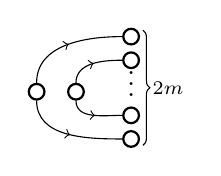
\begin{tikzpicture}
\node [zxopen] (1) at (0,0) {};
\node [zxopen] (2) at (0,1.3) {};
\node [zxopen] (3) at (0,0.3) {};
\node [zxopen] (4) at (0,1) {};
\node [zxopen] (5) at (-0.7,0.6) {};
\node [zxopen] (6) at (-1.2,0.6) {};
\node at (0,0.8) {$\vdots$};
%
\draw [->-]  (5) to [in=180,out=90] (4);
\draw [->-] (5) to [in=180,out=-90] (3);
\draw [->-] (6) to [in=180,out=-90] (1);
\draw [->-] (6) to [in=180,out=90] (2);
%
\draw[decoration={brace,mirror,raise=2pt},decorate]
(1.south east) -- node [right=2pt] {\scriptsize $2m$} (2.north east); 
\end{tikzpicture}
\]
\end{document}
